% Thesis Introduction

\chapter[Introduction]{Introduction}
\label{chap-intro}

\section[Autonomous Unmanned Vehicles]{Autonomous Unmanned Vehicles}

Since the industrial revolution, autonomous machines have become a big contributor to increased human productivity.
From the steam engine and assembly line conveyor belt, autonomous machines take over repetitive, labor intensive tasks and leave human with tasks requiring more attention to details but less labor.
Every year, the list of tasks automated by machines grow bigger.
Vehicles were one of the first few machines predicted to be automated, yet Autonomous Unmanned Vehicles (AUV) just recently became commercially available, although in smaller scales.

With the advent of commercially available small AUV, we can automate tasks such as surveying, sensor network distribution and inspection, which previously require intensive human labor.
Simple surveying with visual, sonar and laser sensor with Unmanned Aerial Vehicles (UAV) have become commercially available.
UAV photography is becoming a booming business, with turn key solution packages.
Enabling photo and movie studios to get aerial footage and pictures without the need for expensive helicopter rentals.
UAV surveying with traditional or modified surveying equipment reduce the cost of surveying sites for constructions or archeological digs.


\section[Seismic AUV] {Deploying seismic microphones with AUV}

\begin{figure}
\centering
\begin{overpic}[width=\columnwidth]{ral2016/intro.pdf}\end{overpic}
\caption{\label{fig:Hetero_overall}
The heterogeneous sensor system presented in this paper: wireless SeismicDarts and a SeismicSpider, both designed for UAV deployment. 
}
\end{figure}

Seismic microphones are used in seismic surveying to find subsurface deposits of natural resources.
Seismic surveying can also be used to identify where earth quakes can happen.
Traditionally, seismic microphones are connected $\SI{2}{\metre}$ or $\SI{3}{\metre}$ apart on a long cable.
The cable is composed of 20 to 30 microphones, and connected to one computer responsible for recording the reflected sound wave.
Several cables can be laid out to cover the entire survey area, so length of cable required is proportional to survey area.
Transporting the cables means increased weight, and they can be difficult to maneuver and deploy on rough terrain.
Surveyors will need to expand a lot of manual labor to deploy these sensors

Recently, nodal sensors with their own recording unit can be deployed, eliminated the need for cabling.
However, these nodal sensors are still deployed and recovered by hand, requiring surveyors to traverse rough terrain multiple times.

Our first use of AUV is to make nodal seismic microphone deployable from an Unmanned Aerial Vehicle (UAV).
Our system can be seen in Fig.~\ref{fig:Hetero_overall}.
The SeismicDart is a dart shaped, wireless capable sensor that can be dropped from a UAV to firmly plant into the ground.
The SeismicSpider is a mobile six legged robot rover with three seismic microphone for legs.
The Spider can be deployed in a clearing where UAVs can access, then walk into more covered area were it's hard for UAV to fly over and deploy SeismicDart.
The system can be utilized to quickly deploy sensor asset for geoscience research~\cite{werner2006deploying} such as
earthquake~\cite{dominici2012micro},
and volcano \cite{nagatani2013volcanic} monitoring,
defense operations~\cite{wu2007efficient},
and wildlife monitoring~\cite{dyo2010evolution,mainwaring2002wireless}. 

\section[Mosquito AUV]{Destructive surveying of mosquito with UAV}

\begin{figure}
	\centering
	\begin{overpic}[width=1\columnwidth]{icra2018/DroneAndNet_v2.pdf}\end{overpic}
	\caption{\label{fig:DroneAndNet}
		A hexacopter UAV carrying a $\SI{48}{\centi\metre} \times \SI{61}{\centi\metre}$ rectangular bug-zapping screen.
		An onboard micro controller monitors the voltage across the screen and records the time, GPS location, humidity, and altitude for each mosquito strike.
		At right are three frames recorded by the onboard camera showing mosquito hits, during the day (top) and at twilight.
		See attachment for videos of flight experiments~\cite{Bhatnagar2018}.
	\vspace{-2em}
	}
\end{figure}

Mosquito-borne diseases kill millions of humans each year~\cite{murray2012global}. 
Because of this threat, governments worldwide track mosquito populations.
Tracking individual mosquitoes is difficult because of their small size, wide-ranging flight, and preference for low-light.
Tracking studies of individual mosquitos have chosen to use small ($\SI{1.2}{\metre} \times \SI{2.4}{\metre}$) indoor regions~\cite{parker2015infrared}, or mating swarms backlit against a solid background~\cite{butail20113d}.

The dominant tools for tracking mosquito populations are stationary traps that are checked at weekly intervals (\textit{e.g.} Encephalitis Vector Surveillance traps and/or gravid traps~\cite{williams2007comparison}). 
Recent research has focused on making these traps smaller, cheaper, and capable of providing real-time data~\cite{chen2014flying,linn2016building}; however, they still rely on attracting mosquitoes to the trap. 
We presents an alternate solution using an electrified bug-zapping screen mounted on an unmanned aerial vehicle (UAV) as shown in Fig.~\ref{fig:DroneAndNet} to seek out the mosquitoes in their habitat.
As the UAV follows a path, it sweeps out a volume of air, temporarily removing all the mosquitoes in this volume.
By monitoring the voltage across this screen, we can track individual mosquito contacts.
UAVs have strict energy budgets, so optimized flight patterns are of crucial importance.
As a consequence, putting the UAV to good use requires methods for computing trajectories that minimize energy consumption along the way, but maximize the total volume of mosquitoes at visited locations.

\section[Drifting sensors]{Surveying underwater with drifting sensors}

\begin{figure}[h]
	\begin{center}
	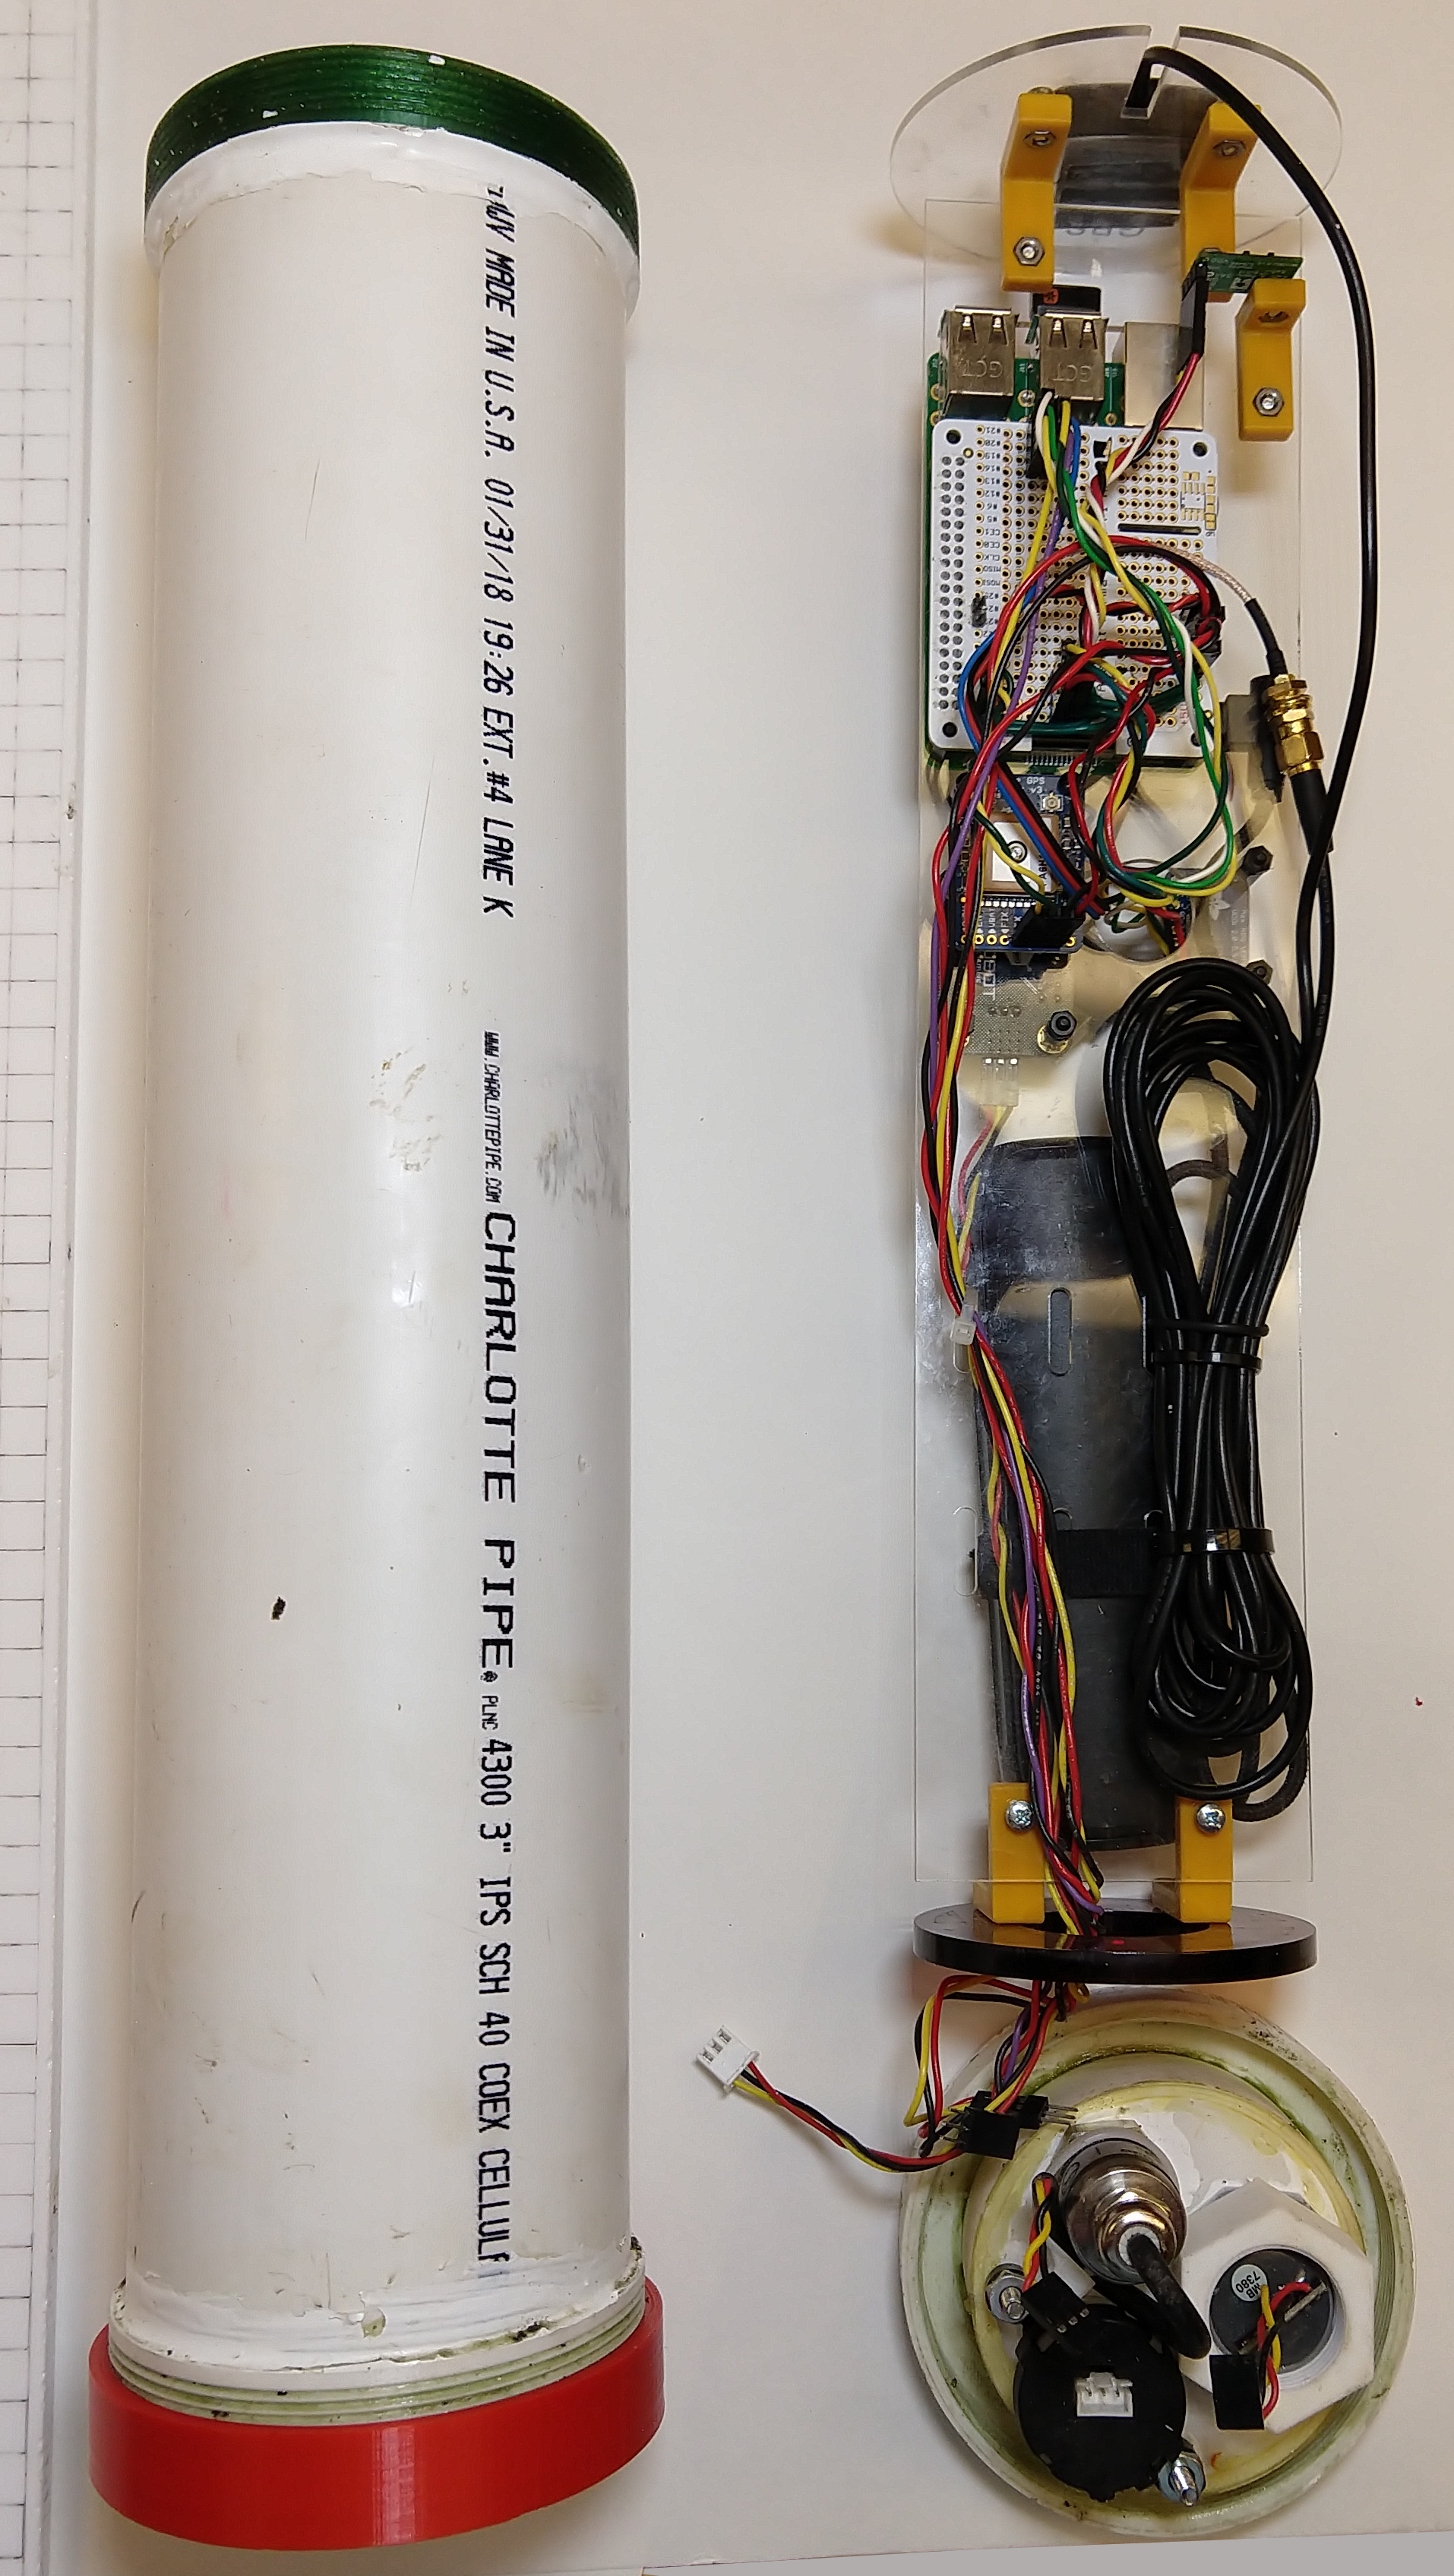
\includegraphics[width=.3\columnwidth]{driftnode/driftnode.jpg}
	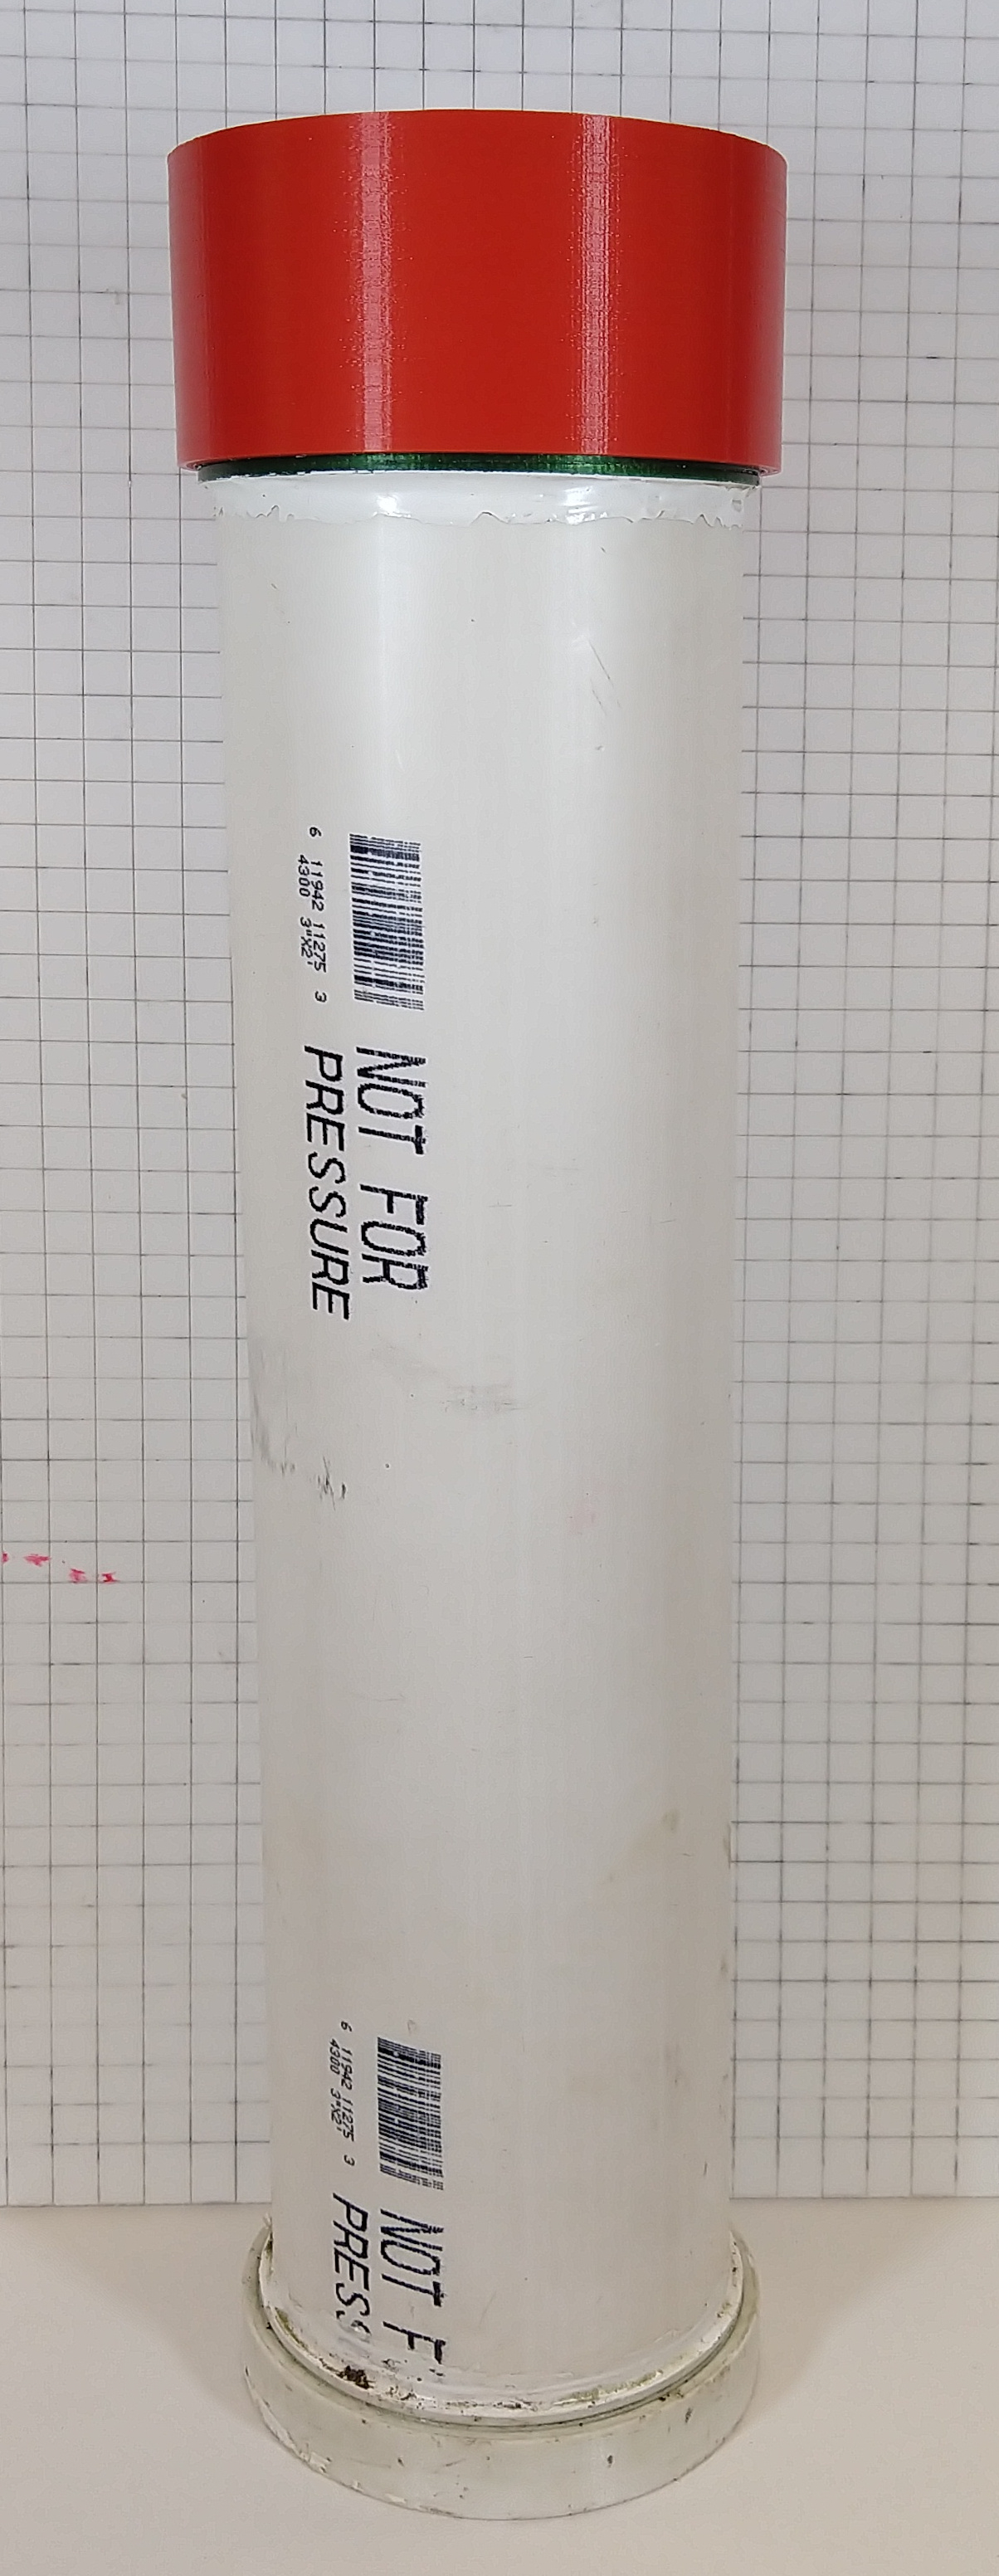
\includegraphics[width=.3\columnwidth]{driftnode/driftnodeassembled.jpg}
	\caption[Driftnode]{
		(Left) driftnode before assembly, the electronics are attached to a center acrylic plate.
		(Right) an assembled driftnode.
	} \label{fig:driftnodeoverview}
	\end{center}
	\vspace{-1em}
\end{figure}

Human know less about the ocean than they do about space.
Because EM waves attenuates quickly in water, it is difficult to deploy wireless sensor network in water for permanent surveying post.
To survey a water surface, a boat with crew needs to be dispatched.
The crew can then manually deploy sensor at each locations within the erea for scientific research.
To monitor an area for border security or fishing enforcements, the crew will need to be deployed periodically.
One crew cannot monitor several area simultaneously, so the man hour needed grew proportionally with area monitored.
This require the need for several crews, or risk security incidence when an area is not monitored.

A wireless sensor network, composed of drifting sensors, deployed temporarily or permanently, can monitor an area for much longer with less labor needed.
A UAV can be used to periodically visit these sensors, collecting their sensor logs and charging them.
We present a basic drifting sensor, originally created by the University of South Carolina \cite{drifterUSC}, as seen in Fig.~\ref{fig:driftnodeoverview}.
The drifting sensor is composed of a suite of basic underwater sensor: an underwater depth sensor, a pressure sensor, a turbidity sensor, 9-axis IMU and GPS location sensor.
Our drifting sensor can broadcast its own wireless access point, which enable an AUV to collect data from the sensor at close range.
